\documentclass{article}
\usepackage[utf8]{inputenc}
\usepackage[T1]{fontenc}
\usepackage{xcolor}
\usepackage{pgfplots}
\pgfplotsset{compat=1.16}
\usepgfplotslibrary{groupplots}
\usetikzlibrary{arrows.meta,arrows}
\usetikzlibrary{backgrounds,calc,bending,backgrounds}

\begin{document}

    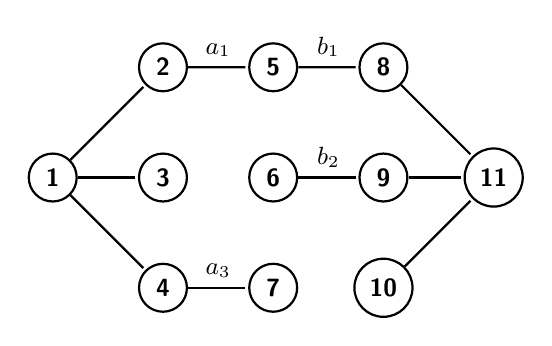
\begin{tikzpicture}[scale=0.7,-,>=stealth',shorten >=1pt,auto,node distance=3cm,
                    thick,main node/.style={circle,draw,font=\sffamily\small\bfseries}]

  \node[main node] (1) at (0,2) {1};
  \node[main node] (2) at (2,4) {2};
  \node[main node] (3) at (2,2) {3};
  \node[main node] (4) at (2,0){4};
  \node[main node] (5) at (4,4){5};
  \node[main node] (6) at (4,2) {6};
  \node[main node] (7) at (4,0){7};
  \node[main node] (8) at (6,4){8};
  \node[main node] (9) at (6,2){9};
  \node[main node] (10) at (6,0){10};
  \node[main node] (11) at (8,2){11};
  \path[every node/.style={font=\sffamily\small}]
  (1) edge node[above] {} (2)
  (1) edge node [left] {} (3)
  (1) edge node [left] {} (4)
  (2) edge node [above] {$a_1$ } (5)
  (4) edge node [above] {$a_3$ } (7)
  (5) edge node [above] {$b_1$ } (8)
  (6) edge node [above] {$b_2$ } (9)
  (8) edge node [left] { } (11)
  (9) edge node [left] { } (11)
  (10) edge node [left] { } (11);
\end{tikzpicture}

\end{document}